%%%%%%%%%%%%%%%%%%%%%%%%%%%%%%%%%%%%%%%%%%%%%%%%%%%%%%%%%%%%%%%%%%%%%%%%
% Uni Duesseldorf
% Lehrstuhl fuer Datenbanken und Informationssysteme
% Vorlage fuer Bachelor-/Masterarbeiten
% Optimiert fuer den Original-Latex-Kompiler LATEX.EXE (LaTeX=>PS=>PDF)
%%%%%%%%%%%%%%%%%%%%%%%%%%%%%%%%%%%%%%%%%%%%%%%%%%%%%%%%%%%%%%%%%%%%%%%%
% Ueberarbeitung für pdflatex (LaTeX=>PDF)
%%%%%%%%%%%%%%%%%%%%%%%%%%%%%%%%%%%%%%%%%%%%%%%%%%%%%%%%%%%%%%%%%%%%%%%%
% Vorlage Changelog:
% 10.09.2015 (Matthias Liebeck): Nummerierung des Inhaltsverzeichnis nun römisch, Beispiel für einen Anhang eingebaut, \raggedbottom hinter sections eingefügt
% 11.07.2018 (Matthias Liebeck): Ersetzung des Bibliographiestils, Einsatz von Biber
% 04.09.2018 (Matthias Liebeck):
%   * Bibtex: unnötige Bibtexfelder beim Rendern ausblenden (thx @ Markus Brenneis)
%   * ngerman: "et al." im BibTeX für drei oder mehr Autoren
%   * Neuer Befehl \sectionforcestartright: Sections immer rechts beginnen (thx @ Philipp Grawe)
%   * ngerman: Deutsche Anführungszeichen im Literaturverzeichnis (thx @ Markus Brenneis)
%   * ngerman: Deutsche Anführungszeichen im Literaturverzeichnis (thx @ Markus Brenneis)
% 16.10.2018 (Matthias Liebeck): Zwei fixes an \sectionforcestartright (thx @ Markus Brenneis)
%%%%%%%%%%%%%%%%%%%%%%%%%%%%%%%%%%%%%%%%%%%%%%%%%%%%%%%%%%%%%%%%%%%%%%%%
%%%% BEGINN EINSTELLUNG FUER DIE ARBEIT. UNBEDINGT ERFORDERLICH! %%%%%%%
%%%%%%%%%%%%%%%%%%%%%%%%%%%%%%%%%%%%%%%%%%%%%%%%%%%%%%%%%%%%%%%%%%%%%%%%
% Geben Sie Ihren Namen hier an:

\newcommand{\bearbeiter}{Norman Nabhan}

% Geben Sie hier den Titel Ihrer Arbeit an:
\newcommand{\titel}{Projektskizze}


% Falls Sie die Arbeit zweiseitig ausdrucken wollen,
% benutzen Sie die folgende Zeile mit
% \AN fuer zweiseitigen Druck
% \AUS fuer einseitigen Druck
\newcommand{\zweiseitig}{\AUS}
% true fuer biber, false fuer klassischen Zitierstil
%\newcommand{\biber}{false}
\newcommand{\biber}{false}

% Falls Sections immer rechts beginnen sollen. Gerade für Masterarbeiten
% interessant. Bei kurzen Bachelorarbeiten eher weniger zu verwenden.
\newcommand{\sectionforcestartright}{false}
%\newcommand{\sectionforcestartright}{true}

% Falls die Arbeit in englischer Sprache verfasst
% werden soll, dann benutzen Sie die folgende Zeile mit
% englisch fuer englische Sprache
% deutsch fuer deutsche Sprache
\newcommand{\sprache}{deutsch}

% Hier wird eingestellt, ob es sich bei der Arbeit um eine Bachelor-
% oder Masterarbeit handelt (unpassendes auskommentieren!):
\newcommand{\arbeit}{Bachelorarbeit}
%~ \newcommand{\arbeit}{Masterarbeit}


%%%%%%%%%%%%%%%%%%%%%%%%%%%%%%%%%%%%%%%%%%%%%%%%%%%%%%%%%%%%%%%%%%%%%%%%
%%%% ENDE EINSTELLUNGEN %%%%%%%%%%%%%%%%%%%%%%%%%%%%%%%%%%%%%%%%%%%%%%%%
%%%%%%%%%%%%%%%%%%%%%%%%%%%%%%%%%%%%%%%%%%%%%%%%%%%%%%%%%%%%%%%%%%%%%%%%

% Die folgende Zeile NICHT EDITIEREN oder loeschen


%%%%%%%%%%%%%%%%%%%%%%%%%%%%%%%%%%%%%%%%%%%%%%%%%%%%%%%%%%%
% Obere Titelmakros. Editieren Sie diese Datei nur, wenn
% Sie sich ABSOLUT sicher sind, was Sie da tun!!!
% (Z.B. zum Abaendern der BA-Vorlage in eine MA-Vorlage)
% Uni Duesseldorf
% Lehrstuhl fuer Datenbanken und Informationssysteme
% Version 2.2 - 2.3.2010
%%%%%%%%%%%%%%%%%%%%%%%%%%%%%%%%%%%%%%%%%%%%%%%%%%%%%%%%%%%
\newcommand{\AN}{twoside}
\newcommand{\AUS}{}


%\newcommand{\englisch}{}
%\newcommand{\deutsch}{\usepackage[german]{babel}}

%% Die folgenden auskommentierten Optionen dienen der automatischen
%% Erkennung des Latex-Kompilers und dem Setzen der davon abhängigen
%% Einstellungen. Bei Problem z.B. mit dem Einbinden von verschiedenen
%% Grafiktypen bei Verwendung von PdfLatex oder Latex, einfach die
%% verschiedenen \usepackage(s) ausprobieren. (Mit diesen Einstellungen
%% funktionierte diese Vorlage bei der Verwenundg von latex.exe als
%% Kompiler bei den meisten Studierenden.)

%\newif\ifpdf \ifx\pdfoutput\undefined
%\pdffalse % we are not running pdflatex
%\else
%\pdfoutput=1 % we are running pdflatex
%\pdfcompresslevel=9 % compression level for text and image;
%\pdftrue \fi

\documentclass[11pt,a4paper, \zweiseitig]{article}
\usepackage{ifthen}


%\usepackage[iso]{umlaute}
\usepackage[utf8]{inputenc}
\usepackage{libertine} % palatino Schriftart
%\usepackage{makeidx} % um ein Index zu erstellen
\usepackage[nottoc]{tocbibind}
\usepackage[T1]{fontenc} %fuer richtige Trennung bei Umlauten
\usepackage{fancybox} % fuer die Rahmen
\usepackage{shortvrb}
\usepackage{url}
\usepackage{xcolor}
\usepackage[colorlinks,citecolor=blue,linkcolor=black]{hyperref} %anklickbares Inhaltsverzeichnis

\ifthenelse{\boolean{\biber}}{
  % only needed for biber
  \usepackage[style=authoryear,natbib=true,backend=biber,mincitenames=1,maxcitenames=2,maxbibnames=99,uniquelist=false,dashed=false]{biblatex}

  % https://tex.stackexchange.com/a/334703/8850
  \AtEveryBibitem{%
    \clearfield{issn}
    \clearfield{isbn}
    \clearfield{doi}
    \clearfield{location}
    \clearlist{location}
    \clearlist{address}

    \ifentrytype{online}{}{% Remove url except for @online
      \clearfield{url}
    }
  }
}
{}%no else

% Falls es bei \citet ein Komma zwischen Name und Jahr gibt:
% https://tex.stackexchange.com/questions/312539/unwanted-comma-between-author-and-year-using-citet-command
% (thx @ Markus Brenneis)
%\DeclareDelimFormat[cbx@textcite]{nameyeardelim}{\addspace}



\ifthenelse{\equal{\sprache}{deutsch}}{
  \usepackage[ngerman]{babel}
  % Bibtex u.a -> et al.
  \ifthenelse{\boolean{\biber}}{
    \DefineBibliographyStrings{ngerman}{
      andothers = {{et\,al\adddot}},
    }
    \newcommand{\references}{Literatur}
  }
  {} % do nothing when not using biber
  \usepackage[autostyle, german=quotes]{csquotes} % Deutsche Anführungszeichen im Literaturverzeichnis (thx @ Markus Brenneis)

}{ \newcommand{\references}{References}}

\usepackage{a4wide} % ganze A4 Weite verwenden



%\ifpdf
%\usepackage[pdftex,xdvi]{graphicx}
%\usepackage{thumbpdf} %thumbs fuer Pdf
%\usepackage[pdfstartview=FitV]{hyperref} %anklickbares Inhaltsverzeichnis
%\else
%\usepackage[dvips,xdvi]{graphicx}
\usepackage{graphicx}

%\fi

\newcommand{\redt}[1] {
  \textcolor{red}{#1}}

\newcommand{\oranget}[1] {
  \textcolor{orange}{#1}}

\newcommand{\purplet}[1] {
  \textcolor{purple}{#1}}

%%%%%%%%%%%%%%%%%%%%%%% Massangaben fuer die Arbeit %%%%%%%%%%%%%%%
\setlength{\textwidth}{15cm}

\setlength{\oddsidemargin}{35mm}
\setlength{\evensidemargin}{25mm}

\addtolength{\oddsidemargin}{-1in}
\addtolength{\evensidemargin}{-1in}

\ifthenelse{\boolean{\biber}}{\addbibresource{references.bib}}{}

%\makeindex
\begin{document}
%\setcounter{secnumdepth}{4} %Nummerieren bis in die 4. Ebene
%\setcounter{tocdepth}{4} %Inhaltsverzeichnis bis zur 4. Ebene

\pagestyle{headings}

\sloppy % LaTeX ist dann nicht so streng mit der Silbentrennung
%~ \MakeShortVerb{\§}

\parindent0mm
\parskip0.5em


{
\textwidth170mm
\oddsidemargin30mm
\evensidemargin30mm
\addtolength{\oddsidemargin}{-1in}
\addtolength{\evensidemargin}{-1in}

\parskip0pt plus2pt

% Die Raender muessen eventuell fuer jeden Drucker individuell eingestellt
% werden. Dazu sind die Werte fuer die Abstaende `\oben' und `\links' zu
% aendern, die von mir auf jeweils 0mm eingestellt wurden.

%\newlength{\links} \setlength{\links}{10mm}  % hier abzuaendern
%\addtolength{\oddsidemargin}{\links}
%\addtolength{\evensidemargin}{\links}

\begin{titlepage}
\vspace*{-1.5cm}
\raisebox{17mm}{
    \begin{minipage}[t]{70mm}
        \begin{center}
            %\selectlanguage{german}
            {\Large INSTITUT FÜR INFORMATIK\\}
            {\normalsize
                Betriebssysteme\\
            }
            \vspace{3mm}
            {\small Universitätsstr. 1 \hspace{5ex} D--40225 Düsseldorf\\}
        \end{center}
    \end{minipage}
}
\hfill
\raisebox{7mm}{
    
\includegraphics[width=130pt]{bilder/HHU_Logo}}
\vspace{14em}

% Titel
\begin{center}
    \baselineskip=55pt
    \textbf{\huge \titel}
    \baselineskip=0 pt
\end{center}

%\vspace{7em}

\vfill

% Autor
\begin{center}
    \textbf{\Large
        \bearbeiter
    }
\end{center}

\vspace{35mm}

% Prüfungsordnungs-Angaben
\begin{center}
%\selectlanguage{german}


\vspace{2em}
\ifthenelse{\equal{\sprache}{deutsch}}{
    \begin{tabular}[t]{ll}
    Datum:& {\today} \\
    
\end{tabular}
\end{center}

\end{titlepage}

}

%%%%%%%%%%%%%%%%%%%%%%%%%%%%%%%%%%%%%%%%%%%%%%%%%%%%%%%%%%%%%%%%%%%%%
\clearpage
\begin{titlepage}
    ~                % eine leere Seite hinter dem Deckblatt
\end{titlepage}
%%%%%%%%%%%%%%%%%%%%%%%%%%%%%%%%%%%%%%%%%%%%%%%%%%%%%%%%%%%%%%%%%%%%%

%%%%%%%%%%%%%%%%%%%%%%%%%%%%%%%%%%%%%%%%%%%%%%%%%%%%%%%%%%%%%%%%%%%%%
% Leerseite bei zweiseitigem Druck
%%%%%%%%%%%%%%%%%%%%%%%%%%%%%%%%%%%%%%%%%%%%%%%%%%%%%%%%%%%%%%%%%%%%%

\ifthenelse{\equal{\zweiseitig}{twoside}}{\clearpage\begin{titlepage}
        ~\end{titlepage}}{}

%%%%%%%%%%%%%%%%%%%%%%%%%%%%%%%%%%%%%%%%%%%%%%%%%%%%%%%%%%%%%%%%%%%%%


%%%%%%%%%%%%%%%%%%%%%%%%%%%%%%%%%%%%%%%%%%%%%%%%%%%%%%%%%%%%%%%%%%%%%
% Leerseite bei zweiseitigem Druck
%%%%%%%%%%%%%%%%%%%%%%%%%%%%%%%%%%%%%%%%%%%%%%%%%%%%%%%%%%%%%%%%%%%%%
\ifthenelse{\equal{\zweiseitig}{twoside}}
{\clearpage\begin{titlepage}~\end{titlepage}}{}
%%%%%%%%%%%%%%%%%%%%%%%%%%%%%%%%%%%%%%%%%%%%%%%%%%%%%%%%%%%%%%%%%%%%%
\clearpage \setcounter{page}{1}
\pagenumbering{roman}
\setcounter{tocdepth}{2}
\tableofcontents

%\enlargethispage{\baselineskip}
\clearpage
%%%%%%%%%%%%%%%%%%%%%%%%%%%%%%%%%%%%%%%%%%%%%%%%%%%%%%%%%%%%%%%%%%%%%
% Leere Seite, falls Inhaltsverzeichnis mit ungerader Seitenzahl und
% doppelseitiger Druck
%%%%%%%%%%%%%%%%%%%%%%%%%%%%%%%%%%%%%%%%%%%%%%%%%%%%%%%%%%%%%%%%%%%%%
\ifthenelse{ \( \equal{\zweiseitig}{twoside} \and \not \isodd{\value{page}} \)}
{\pagebreak \thispagestyle{empty} \cleardoublepage}{\clearpage}


% Kapitel soll bei doppelseitigem Druck immer auf der rechten (ungeraden) Seite anfangen (thx @ Philipp Grawe)
% https://tex.stackexchange.com/a/223387
\ifthenelse{\boolean{\sectionforcestartright}}
{\let\oldsection\section % Store \section in \oldsection
    \renewcommand{\section}{\cleardoublepage\oldsection}}
{}
\pagenumbering{arabic}
\setcounter{page}{1}

%%%%%%%%%%%%%%%%%%%%%%%%%%%%%%%%%%%%%%%%%%%%%%%%%%%%%%%%%%%%%%%%%%%%%%%%
%%%% BEGINN TEXTTEIL %%%%%%%%%%%%%%%%%%%%%%%%%%%%%%%%%%%%%%%%%%%%%%%%%%%
%%%%%%%%%%%%%%%%%%%%%%%%%%%%%%%%%%%%%%%%%%%%%%%%%%%%%%%%%%%%%%%%%%%%%%%%

%%%%%%%%%%%%%%%%%%%%%%%%%%%%%%%%%%%%%%%%%%%%%%%%%%%%%%%%%%%%%%%%%%%%%%%%
% Text entweder direkt hier hinein schreiben oder, im Sinne der
% besseren Uebersichtlich- und Bearbeitbarkeit mittels \input die
% einzelnen Textteile hier einbinden.
%%%%%%%%%%%%%%%%%%%%%%%%%%%%%%%%%%%%%%%%%%%%%%%%%%%%%%%%%%%%%%%%%%%%%%%%

\section{Einführung}\raggedbottom

\subsection{Motivation}
Im Rahmen der Projektarbeit soll ein verteilter \textit{in-memory storage} auf Basis von Apache Plasma entwickelt werden. Dieser verteilte Speicher soll in der Lage sein, große Datenmengen im Sinne von \textit{Big Data} zu speichern und zur Verfügung zu stellen.
 
Plasma ist Teil des Apache Arrow Projekts. Dieses Projekt beschreibt sein Einsatzgebiet wie folgt:
\begingroup
\addtolength\leftmargini{0.1in}
\begin{quote}
	``Apache Arrow defines a language-independent columnar memory format for flat and hierarchical data, organized for efficient analytic operations on modern hardware like CPUs and GPUs. The Arrow memory format also supports zero-copy reads for lightning-fast data access without serialization overhead.''\cite{Foundation}
\end{quote}
\endgroup
Der Zugriff erfolgt hierbei über Bibliotheken in diversen Programmiersprachen.
Hierbei sei zu beachten, dass Plasma selbst nicht als verteilte Anwendung konzipiert ist. Zwar können mehrere Instanzen auf einem Computer gestartet werden, jedoch verfügt Plasma über kein Protokoll, um mehrere Instanzen über ein Netzwerk zu verbinden. Somit ist auch der Speicher nicht verteilt und jeweils nur auf einem Computer verfügbar.

\subsection{Ziel}
Um die oben genannte Problematik zu lösen, soll ein Protokoll entwickelt werden, welches es ermöglicht mehrere Instanzen zu einem Netzwerk Cluster zu verbinden. Dieses Overlay-Netzwerk wird in Java entwickelt. Wie in Abbildung \ref{fig_Architektur} dargestellt, sind alle Komponenten miteinander verbunden. Wobei jeder Node und der Dispatcher jeweils eine direkte Verbindung zu allen anderen Komponenten des Netzwerks besitzt. Wenn Daten gespeichert werden sollen, entscheidet der Dispatcher, welcher Node für die Daten verantwortlich ist. Der Dispatcher nutzt Redis zur Datenhaltung.

\begin{figure}[htb]
	\begin{center}
		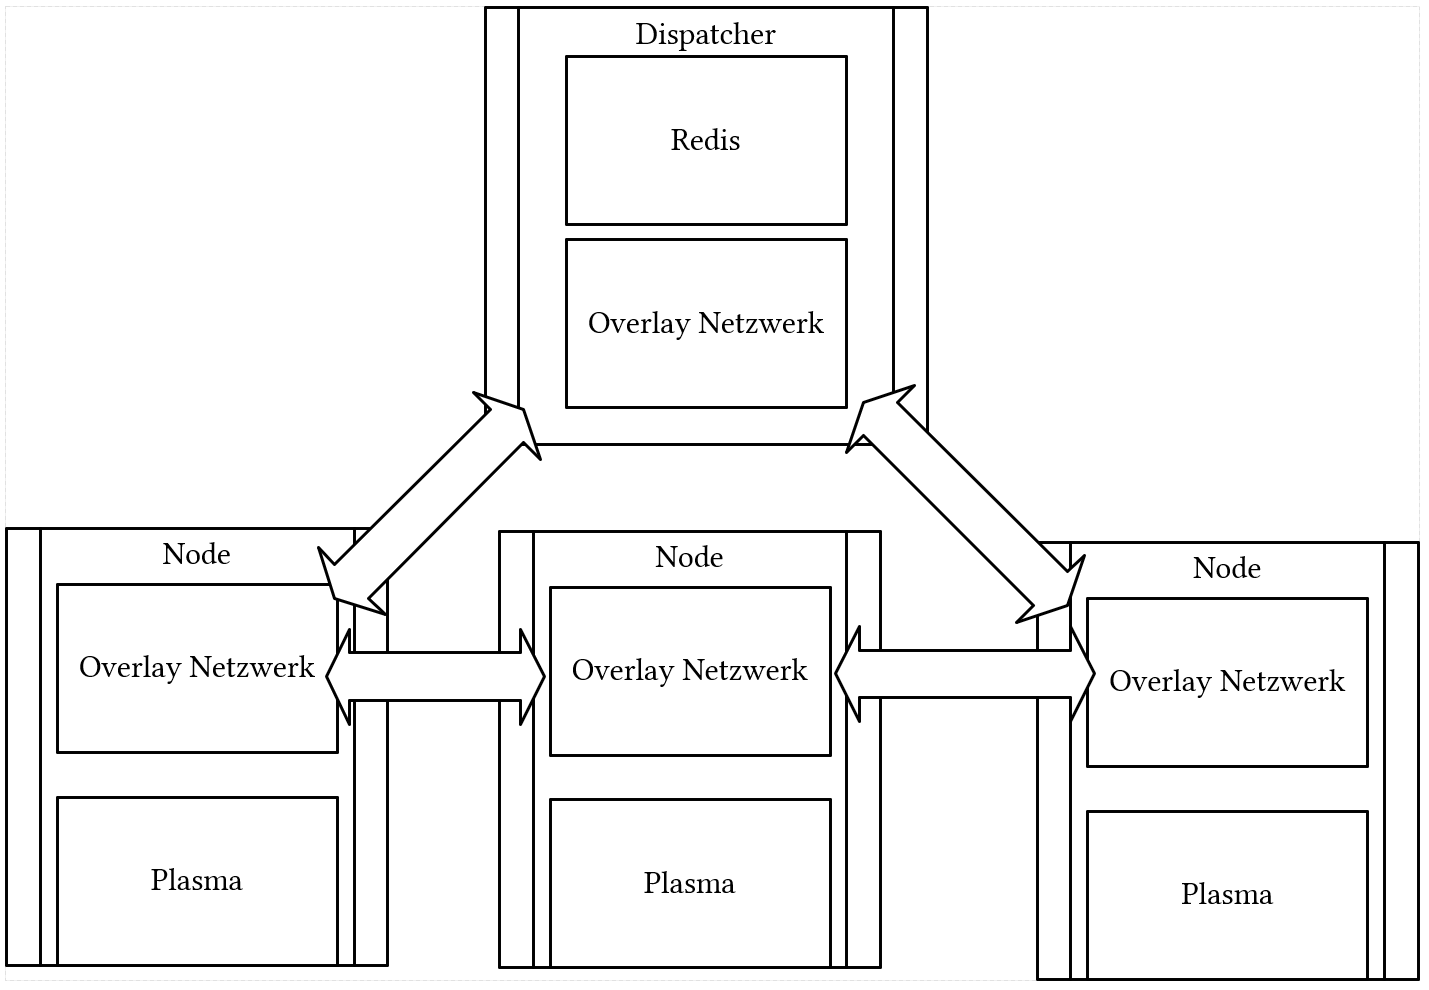
\includegraphics[width=0.8\textwidth]{bilder/Architektur.png}
		\caption{Skizze der angedachten Architektur.}\label{fig_Architektur}
	\end{center}
\end{figure}


\pagebreak
\section{Projektstufen}\raggedbottom
Die Projektarbeit gliedert sich in verschiedene, aufeinander folgende Phasen. Die Projektarbeit beginnt mit einem theoretischen Teil und endet mit einem praktischen Teil.
\subsection{Theoretischer Teil}
Dieser Teil beginnt mit der Anforderungsanalyse. Die hier beschriebene Software soll in ein bereits existierendes System integriert werden. Somit muss die Kompatibilität zu den bereits existierenden Komponenten in Form von Soft- und Hardware gewährleistet sein.
Darauf folgt der Entwurf der Anwendungsfälle. Hierbei gilt es Funktionalitäten zu beschreiben, die zwingend notwendig sind. Ergänzend dazu können noch weitere Funktionalitäten festgelegt werden, die zwar wünschenswert wären, aber nicht zwingend erforderlich sind. Danach muss die Architektur festgelegt und spezifiziert werden, um die Anwendungsfälle zu erfüllen. Verschiedene Lösungsansätze sollen beschrieben und verglichen werden.
\subsection{Praktischer Teil}
Basierend auf der Spezifikation werden die Komponenten implementiert. Zusätzlich sollen Tests und eine Dokumentation des Quellcodes erstellt werden. Die so erstellte Lösung soll in Hinblick auf wichtige Metriken wie IOPs, Bandbreite, Latenz etc. evaluiert werden.

%%%%%%%%%%%%%%%%%%%%%%%%%%%%%%%%%%%%%%%%%%%%%%%%%%%%%%%%%%%%%%%%%%%%%%%%
%%%% ENDE TEXTTEIL %%%%%%%%%%%%%%%%%%%%%%%%%%%%%%%%%%%%%%%%%%%%%%%%%%%%%
%%%%%%%%%%%%%%%%%%%%%%%%%%%%%%%%%%%%%%%%%%%%%%%%%%%%%%%%%%%%%%%%%%%%%%%%

\clearpage

% Entfernen Sie das Kommentar aus der nachfolgenden Zeile, falls Sie einen Anhang in der Arbeit verwenden wollen. Beachten Sie, dass Sie sich im Verlauf der Arbeit mit \ref{...} (z.B. \ref{anhang:zusatz1}) auf den Anhang beziehen.
%\input{anhang}

\ifthenelse{\boolean{\biber}}{ %with biber do
	\DeclareNameAlias{sortname}{first-last}
	\printbibliography[heading=bibintoc, title=\references]
}{ %without biber do
	\bibliography{references}
	\bibliographystyle{IEEEtran}
}
%\vspace*{\fill}

\clearpage

\listoffigures

%\listoftables

%\pagebreak

%\printindex
\end{document}
